% !TeX root = ../main.tex
% Add the above to each chapter to make compiling the PDF easier in some editors.


\chapter{Introduction}\label{chapter:introduction}

Gesellschaft für Anlagen- und Reaktorsicherheit (GRS) conducts research and analysis in its fields of reactor safety, radioactive waste management,radiation and environmental protection. GRS is a leading expert organization in the field of radioactive waste management and nuclear safety.

The company consists of multiple management and scientific departments where each department is responsible for its specific fields. Working together the company has developed numerous different numerical applications and packages for the needs of nuclear safety analysis for the past 40 years. Bellow one can see the list of the  main scientific applications developed by GRS.
 
\begin{itemize}
	\item ASTEC: integral code for determination of the source term during core meltdown for the primary circuit and containment of LWRs
	\item ATHLET: thermohydraulic safety analyses for the primary circuit of  LWRs
	\item ATHLET-CD: analyses of accidents with core meltdown and fission product release for LWRs
	\item ATLAS: analysis simulator for interactive handling and visualisation of several computer codes
	\item COCOSYS: analyses of severe incidents in the containment of LWRs
	\item DORT/TORT: solution of time-dependant neutron transport equations for 2D/3D transients analyses
	\item QUABOX/CUBBOX: 3-D neutron kinetics core model
	\item SUSA: uncertainty and sensitivity analyses
	\item TESPA-ROD: core rod code for design basis accidents
\end{itemize}


Some applications can work together or with other external libraries and applications during a simulation with the aim of solving some multi-physical problems. Figure \ref{fig:applications} schematically shows an example of application coupling for an involved severe accident simulation.\par

As one can imagine each of those applications listed above needs a numerical solver to perform simulations. [solvers fast and parallel] Moreover, each scientific group has to keep developing and maintaining their own solvers which can be seen at the first glance as a work duplication. For that reason GRS made a decision to develop a so-called Numerical Toolkit (NuT) which had to become a universal collection of different and highly efficient numerical solvers. [That idea is not new and it has been use quite long time ago... something about PetSc]\par

\begin{figure}[htpb]
  \centering
  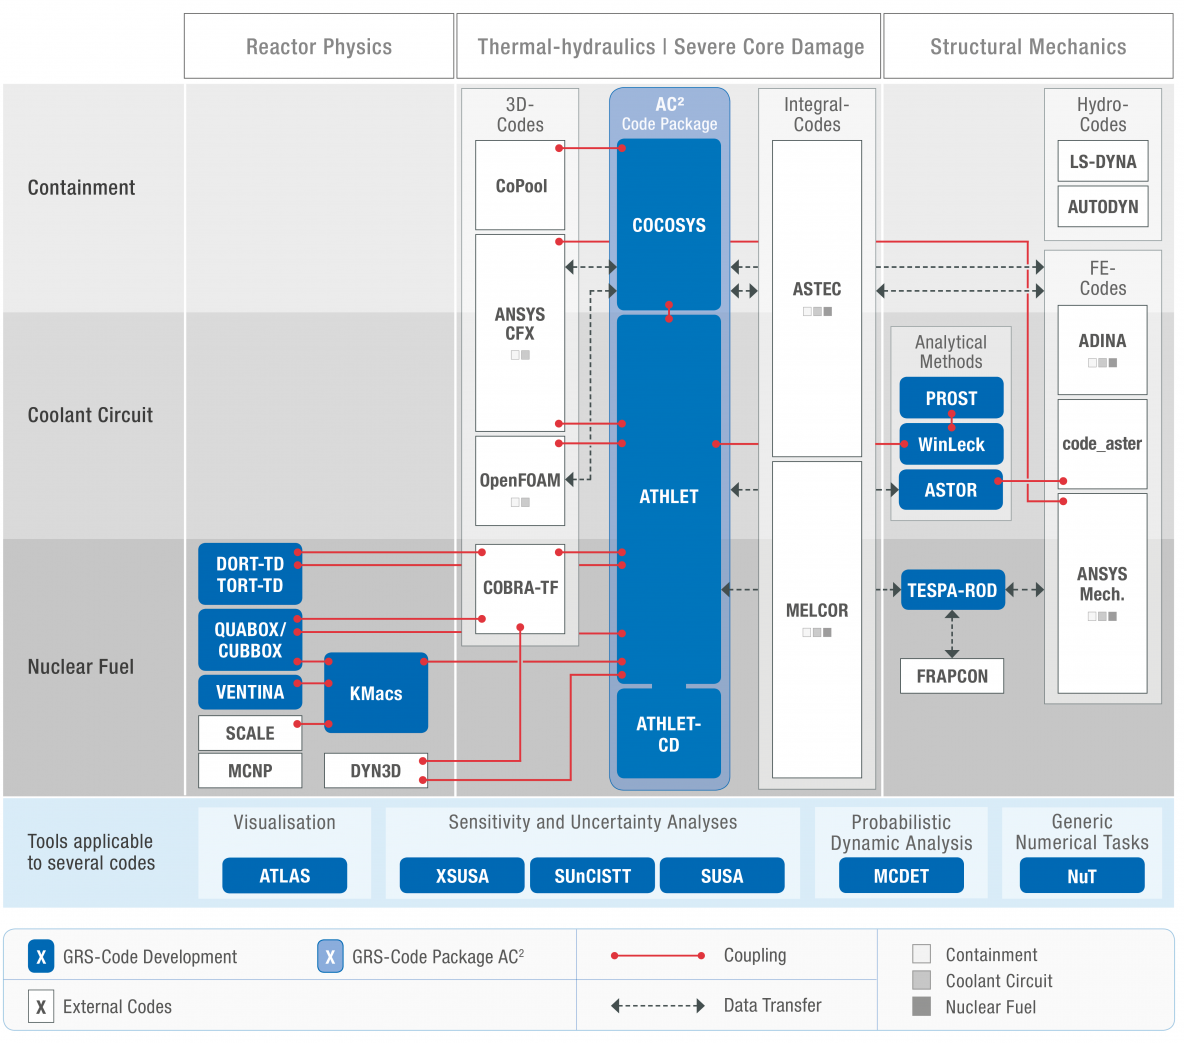
\includegraphics[width=0.8\textwidth]{figures/grs-application-coupling.png}
  \caption{An example of application coupling} \label{fig:applications}
\end{figure}



\section{Newton's method, Jacobian, Coloring}
In some cases the Jacobian matrix has to be computed during time integration for some advanced time integration schemes. These derivative matrices can be estimated through finite
difference approximations or computed exactly, within the limits of machine precision,
through automatic differentiation (AD) [reference]. In this study we will focus only on finite difference approximation technique since it is currently used in all GRS applications.\par 
When a system of equations is sparse it also means that some equations within the system do not depend on each other.The problem of finding independent sets of equations within a sparse system is well known. It was also well studied for parallel Gauss Seidel algorithm also known as Red-Black Gauss Seidel where it is also necessary to find as many as possible independent equations in order to increase concurrency of the algorithm [some reference]. In general this problem is called "matrix partitioning problem" or "coloring" where an individual "color" is assigned to a set of independent equations. It is worth noticing while there is no dependence within a color the colors themselves have dependency between each other. It means that we can perform parallel computations within a color but we have to move from color to color sequentially. It is obvious that a coloring algorithm has to find the least number of colors as possible to achieve better parallel performance.\par

The most comprehensive study in the filed of different graph coloring heuristics has been recently done by Assefaw Hadish Gebremedhin, Fredrik Manne and Alex Pothen in their paper "What Color Is Your Jacobian? Graph Coloring for Computing Derivatives" [reference]. The authors summarized different matrix partitioning problems over the last 20 years and proposed a unifying algorithmic framework for type of problems.\par

Due to specifics of the software architecture the server side (NuT) is responsible to perform matrix partitioning since only sparsity pattern is required for graph coloring [and the server has much more resources (processes) to perform this task in parallel]. However, Jacobian matrix evaluation happens on the client side since the host application has enough information about underlying PDE discretization. Having computed a color, perturbation of a set of independent equations using finite differences, the client sends the result back to the server and continue further. Having received the color, the result of perturbation, the server comes back to the listening state since it cannot proceed with the current task without the full matrix.\par

The most distinguishing thing in case of Jacobian matrix partitioning problem is that sizes of colors, the number of independent equations within a set, are not equal and getting smaller. For example, the first color usually contains the largest amount of equations whereas the last one is significantly smaller in size and can contain only few equations. There are at least 10 different techniques to perform graph coloring and all of them are based on different heuristics [reference]. But all of them lead to the same effect described above. To demonstrate this, let us consider an example of a sparse matrix J $\in$ $\mathbb{R}^{5x5}$. \par
\[
J = 
\begin{bmatrix}
    j_{11} & j_{12} & 0      & 0      & j_{15}\\
    0      & 0      & j_{23} & 0      & 0     \\
    0      & j_{32} & 0      & j_{34} & 0     \\
    j_{41} & 0      & 0      & 0      & 0     \\
    0      & 0      & 0      & j_{54} & j_{55}\\
\end{bmatrix}
\]
\par
We are going to find \textit{structurally orthogonal} columns, columns that do not have a nonzero element in a common row, and group them together. It can be seen that columns 1, 3 and 4 are structurally orthogonal and we can "compress" them. The further analysis shows the rest of the columns, namely: 2 and 5, are not orthogonal and cannot be grouped together. As the result we can represent matrix J in the following compressed way:
\par
\[
J = 
\begin{bmatrix}
    {\color{red}j_{11}} & {\color{blue}j_{12}} & j_{15}\\
    {\color{red}j_{23}} & {\color{blue}0}      & 0     \\
    {\color{red}j_{34}} & {\color{blue}j_{32}} & 0     \\
    {\color{red}j_{41}} & {\color{blue}0}      & 0     \\
    {\color{red}j_{54}} & {\color{blue}0}      & j_{55}\\
\end{bmatrix}
\]
\par
As it can be observed the first, red color contains 6 elements as the size of the matrix and can be simultaneously computed through one finite difference operation. The blue and black colors have only 2 elements each and it is only one third of the column vector size. In some cases sizes of colors can get smaller quite fast.\par

Another illustrative example can be seen in figure [reference] where a 100 by 100 Jacobian matrix is compressed to a 100 by 28 matrix by grouping together nonzero elements in a set of structurally orthogonal columns into a single column. Figure [reference] shows another view on the same results [reference]. The bar chart represents sizes of columns after compression.\par

\begin{figure}[htpb]
  \centering
  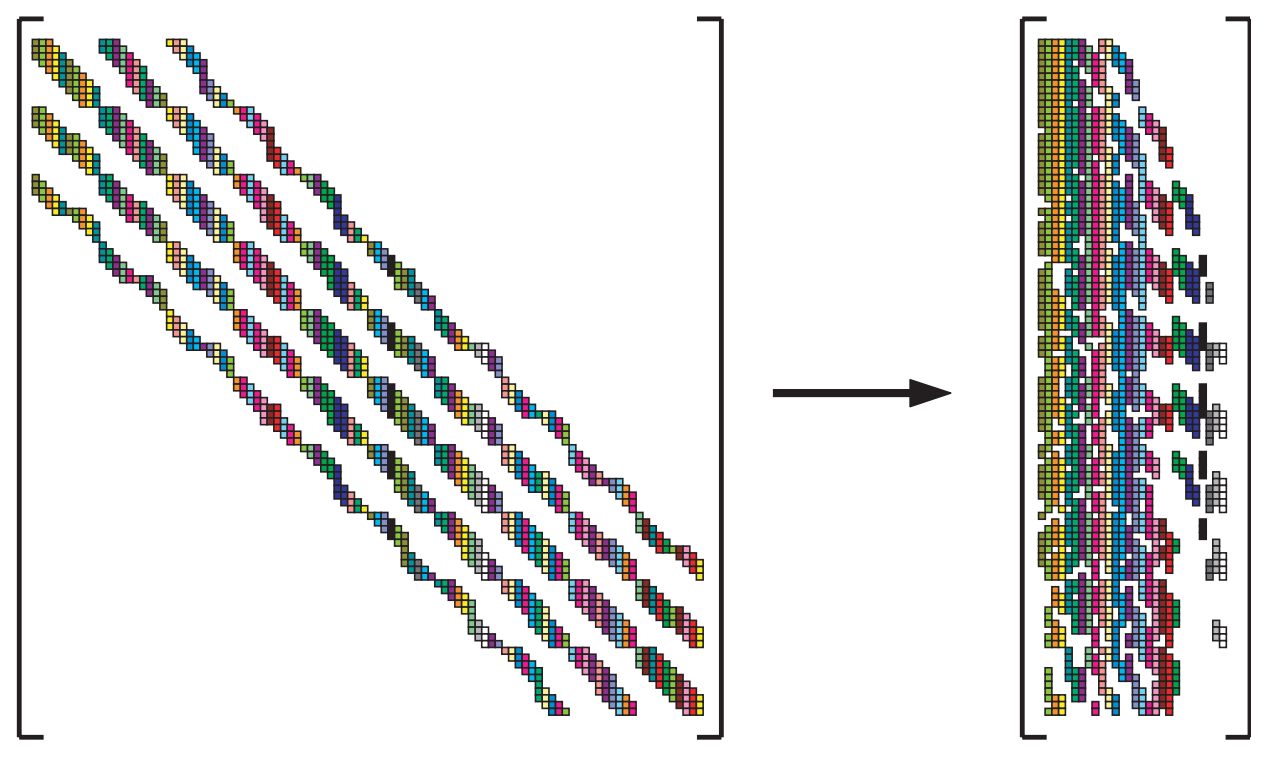
\includegraphics[width=0.8\textwidth]{figures/matrix-compression.png}
  \caption{Matrix Compression} \label{fig:applications}
\end{figure}
\par

\begin{figure}[htpb]
  \centering
  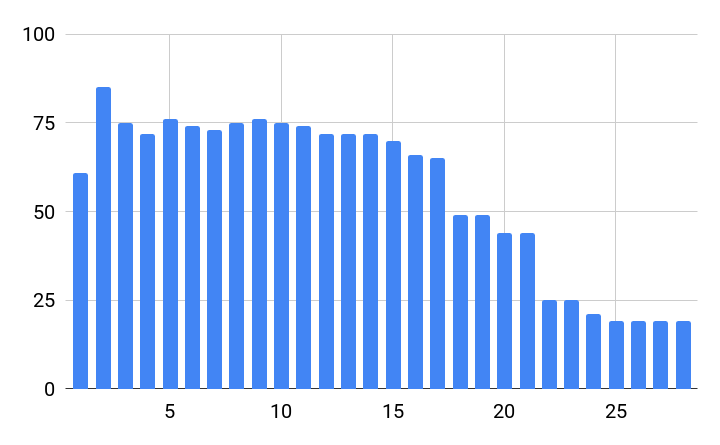
\includegraphics[width=0.8\textwidth]{figures/matrix-compression-2.png}
  \caption{Matrix Compression} \label{fig:applications}
\end{figure}
\par



The effect of color size reduction is the particularly field of interest in this study because it determines the communication pattern between the client and server. It is well known that sending small messages can lead to performance deterioration due to not full resource utilization. In this case we consider the network bandwidth as the main resource.

\emph{example of jacobian evaluation}
\par


 

 and there exist several algorithms which can tackle it, namely: [reference to the book]

The coloring technique 